\documentclass[a4j,twocolumn]{jarticle}
\usepackage[utf8]{inputenc}
\usepackage[cmex10]{amsmath}
\usepackage{amssymb,verbatim}
\usepackage[dvipdfmx]{graphicx}
\usepackage{mathrsfs}
\usepackage{here}
\usepackage{tabularx}
\usepackage{listings,jvlisting}
\usepackage{geometry}
\geometry{left=20mm,right=20mm,top=20mm,bottom=20mm}
\fontsize{14pt}{10pt}\selectfont
\def \figref #1{\figurename\ref{#1}}
\def \tbref #1{\tablename\ref{#1}}
\def \equref #1{式(\ref{#1})}
%\vspace{-20cm}
\title{\vspace{-2em}B16 コヒーレント状態を用いた通信の古典通信容量\\
\vspace{0.5cm}
\normalsize{Classical Capacity for Communication with coherent states}}
\date{}
\pagestyle{empty}
\author{量子情報数理研究室\hspace{50mm}米沢将}
\begin{document}
\maketitle
\thispagestyle{empty}
\section{はじめに}
本発表では,コヒーレント状態を用いて通信を行う際の通信容量について調べる.又,増幅器の効果についても評価を行う.

\section{通信路}
通信路に入力される記号$\{a_1,a_2,…,a_r\}$の集合$A_c$を入力アルファベットと呼ぶ.また,通信路から出力される記号$\{b_1,b_2,…,b_r\}$の集合$A_r$を出力アルファベットと呼ぶ.
ここで,$a_i$が入力された時に$b_j$が出力される条件付き確率$P(b_j|a_i)$を要素とする行列$T$を通信路行列と呼ぶ.

通信路の例として,2元対称通信路について説明する.
2元対称通信路の通信路行列は以下のようにあらわすことができる.
$$
T=\begin{bmatrix}
1-p&p\\
p&1-p
\end{bmatrix}
(0≦p≦1)$$ 
すなわち,通信路に$0$が入力されると確率 $1-p$で$0$が出力され,確率$p$で$1$が出力される.
一方$1$が入力されると確率$p$で$0$が出力され,確率$1-p$で$1$が出力される.
% これを通信路線図を用いて書くと\figref{Fig2_1}のように書くことができる.

%     \begin{figure}[H]
%         \centering   
%         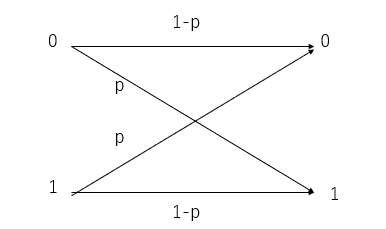
\includegraphics[width=0.4\textwidth]{img/Fig1.png}
%         \caption[sample image (png)]{通信路線図}
%         \label{Fig2_1}
%     \end{figure}


\section{エントロピーと通信容量}
通信容量は,通信路で伝達できる最大の($1$記号当りの)情報量のことである.
通信容量$C$は次式によって与えられることが知られている.
\begin{equation}\label{Cap}
C=\max_{P_X}I(X;Y)  
\end{equation}
ここで,$\max_{P_X}$は先験確率$P_X$を動かして最大値を求めることを意味している.
すなわち通信容量は相互情報量I(X;Y)を$P_X$で最大化したものとなっている.相互情報量は,出力$Y$を知ったときに得る$X$に関する情報量のことで,通信路で伝達される情報量を表している.



相互情報量について詳しく見るために,エントロピーについて説明する.
エントロピーとは確率変数$X$に関する曖昧さを表す量で,
$$
H(X)=-\sum_xP_X(x)\log P_X(x)
$$
によって求めることができる.
条件付きエントロピーは,
$Y$の値を知った時に$x$に関して残る平均の曖昧さを表す量で,
次式によって計算することができる.
$$
H(X|Y)=\sum_xP_Y(y)H(X|Y=y)$$
$$
H(X|Y=y)=-\sum_xP(x|y)\log P(x|y)
$$
これらの式を用いて相互情報量は
$$
I(X;Y)=H(X)-H(X|Y)
$$
と定義される.
条件付きエントロピー$H(X|Y)$は,$Y$の値を知った時に$X$に関して残る平均の曖昧さ
を表している.したがって$H(X)$から$H(X|Y)$を引くと$Y$の値を知ることにより消えた$X$の曖昧さになる.
すなわち相互情報量は,出力$Y$を知ったときに得る$X$に関する情報量となっている.なお,
$H(Y)$から$H(Y|X)$を引いても相互情報量$I(X|Y)$が得られることが知られている.
% \figref{Fig3_1}は相互情報量とエントロピーの関係を表している.
%     \begin{figure}[H]
%         \centering   
%         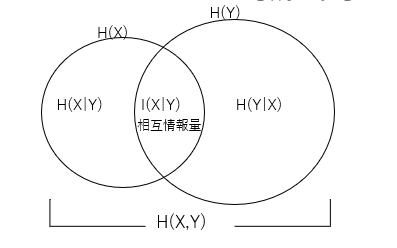
\includegraphics[width=0.5\textwidth]{img/Fig2.png}
%         \caption[sample image (png)]{相互情報量とエントロピーの関係}
%         \label{Fig3_1}
%     \end{figure}

2元対称通信路の通信容量について計算する.
式(\ref{Cap})において,最適な$P_X$は,$P_X(0)=P_X(1)=1/2$となることが知られているので,
この事実を使って通信容量を計算すると次式を得る.
\begin{equation}\label{C2}
  C=1+p\log_2p+(1-p)\log_2(1-p)  
\end{equation}

\section{コヒーレント状態を用いた通信}\label{cohTrns}
複素振幅αを持つ光の状態をコヒーレント状態と呼ぶ.コヒーレント状態$|\alpha\rangle$は次式で与えられる.
\begin{equation}
\begin{split}
|\alpha\rangle&=\sum_nC_n|n\rangle \\
C_n&=e^{-|\alpha|^2/2}\frac{\alpha^n}{\sqrt{n!}}
\end{split}
\end{equation}
以下,$\alpha$を実数として,コヒーレント状態 $|\alpha\rangle$,$|-\alpha\rangle$を用いた通信について考えることとする.この通信では,$0$に対して$|-\alpha\rangle$を,$1$に対して$|\alpha\rangle$を送信する.
受信者はホモダイン測定を行い,その測定値に対してしきい値処理をおこなって$0$または$1$を出力する.ホモダイン測定では,コヒーレント状態の複素振幅$\alpha=x+iy$の$x$成分が測定される.
    \begin{figure}[H]
        \centering   
        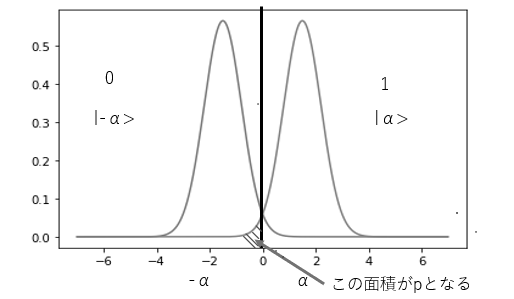
\includegraphics[width=0.5\textwidth]{img/Fig3.png}
        \caption[sample image (png)]{コヒーレント状態をホモダイン測定した場合の出力の確率分布}
        \label{Fig4_1}
    \end{figure}
\figref{Fig4_1}は,コヒーレント状態$\alpha$と$-\alpha$の測定値の確率分布のグラフを表している.この分布はそれぞれ分散$1/4$の正規分布となっている.
そして,閾値を$0$に設定し測定値が$0$より小さい場合は$0$,大きい場合は$1$を受信したと判断する.
したがって,この通信路は2元対称通信路となり,\figref{Fig4_1}の斜線部の面積が誤り確率$p$を表している.
したがって,$p$は,
$$
p=\int_{-\infty}^{x_0}f(x)dx
$$
で計算できる.この積分は累積分布関数を用いて求めることができる.この$p$を用いて式(\ref{C2})を計算すれば
通信容量が得られる.
\figref{Fig4_3}は,通信容量のグラフを表しており,横軸は$\alpha$,縦軸は通信容量となっている.
  \begin{figure}[H]     
  \centering   
  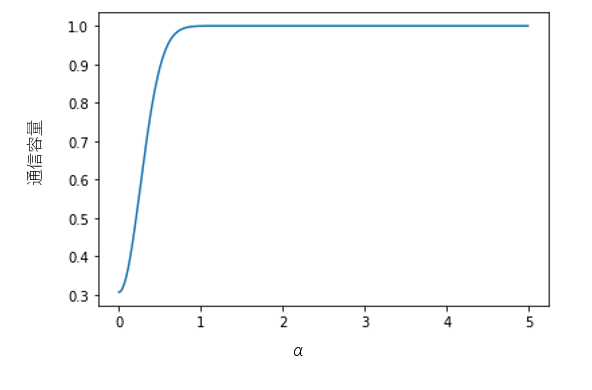
\includegraphics[width=0.5\textwidth]{img/Fig5.png}
\caption[sample image (png)]{$\alpha$の変化で変わる通信容量}     \label{Fig4_3}
\end{figure}
\section{減衰-増幅通信路}
透過率$\lambda$の減衰通信路を使って,コヒーレント状態$|\alpha\rangle$を送信する場合,受信器ではコヒーレント状態
$|\sqrt{\lambda}\alpha\rangle$を得る.一方,減衰通信路の中間地点に増幅器を設置する時,増幅器で雑音が混入するため受信器で受信される状態はコヒーレント状態ではなくなる.この状態を測定すると,平均$\pm \sqrt[4]{\lambda}\alpha$,分散$\frac 34-\frac{\sqrt{\lambda}}{2}$の正規分布が得られる.これらの事実より,第\ref{cohTrns}章と同様にして通信容量を計算することができる.
\figref{Fig5_2},\figref{Fig5_5}は,減衰通信路の透過率がそれぞれ$\lambda=0.1,0.6$の時の通信容量のグラフを表している.実線は増幅器ありの場合,点線は増幅器なしの場合のグラフである.グラフの横軸は送信信号の振幅値$\alpha$ を表し,縦軸は通信容量を表している.

    \begin{figure}[H]
        \centering   
        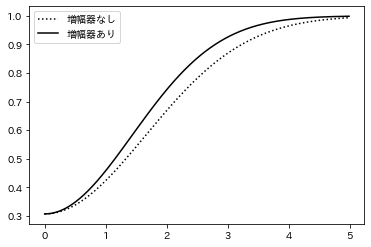
\includegraphics[width=0.4\textwidth]{img/Fig5_2.png}
        \caption[sample image (png)]{$\lambda=0.1$のときの通信容量の変化}
        \label{Fig5_2}
    \end{figure}
    
    \begin{figure}[H]
        \centering   
        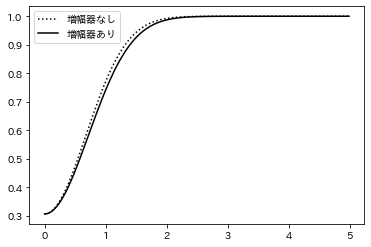
\includegraphics[width=0.4\textwidth]{img/Fig5_5.png}
        \caption[sample image (png)]{$\lambda=0.6$のときの通信容量の変化}
        \label{Fig5_5}
    \end{figure}

\section{まとめ}
コヒーレント状態を用いた2元対称通信路の通信容量の計算を行った.また,減衰通信路を用いた通信を行う場合も考察し,増幅器を設置する効果を確認した.


\begin{thebibliography}{9}
\bibitem{imai}
今井 秀樹,情報・符号・暗号の理論,コロナ社,2004 

\bibitem{inoue}
井上恭,工学系のための量子工学,森北出版株式会社,2020 
\end{thebibliography}
\end{document}
